\documentclass{article}\usepackage[]{graphicx}\usepackage[]{color}
%% maxwidth is the original width if it is less than linewidth
%% otherwise use linewidth (to make sure the graphics do not exceed the margin)
\makeatletter
\def\maxwidth{ %
  \ifdim\Gin@nat@width>\linewidth
    \linewidth
  \else
    \Gin@nat@width
  \fi
}
\makeatother

\definecolor{fgcolor}{rgb}{0.345, 0.345, 0.345}
\newcommand{\hlnum}[1]{\textcolor[rgb]{0.686,0.059,0.569}{#1}}%
\newcommand{\hlstr}[1]{\textcolor[rgb]{0.192,0.494,0.8}{#1}}%
\newcommand{\hlcom}[1]{\textcolor[rgb]{0.678,0.584,0.686}{\textit{#1}}}%
\newcommand{\hlopt}[1]{\textcolor[rgb]{0,0,0}{#1}}%
\newcommand{\hlstd}[1]{\textcolor[rgb]{0.345,0.345,0.345}{#1}}%
\newcommand{\hlkwa}[1]{\textcolor[rgb]{0.161,0.373,0.58}{\textbf{#1}}}%
\newcommand{\hlkwb}[1]{\textcolor[rgb]{0.69,0.353,0.396}{#1}}%
\newcommand{\hlkwc}[1]{\textcolor[rgb]{0.333,0.667,0.333}{#1}}%
\newcommand{\hlkwd}[1]{\textcolor[rgb]{0.737,0.353,0.396}{\textbf{#1}}}%

\usepackage{framed}
\makeatletter
\newenvironment{kframe}{%
 \def\at@end@of@kframe{}%
 \ifinner\ifhmode%
  \def\at@end@of@kframe{\end{minipage}}%
  \begin{minipage}{\columnwidth}%
 \fi\fi%
 \def\FrameCommand##1{\hskip\@totalleftmargin \hskip-\fboxsep
 \colorbox{shadecolor}{##1}\hskip-\fboxsep
     % There is no \\@totalrightmargin, so:
     \hskip-\linewidth \hskip-\@totalleftmargin \hskip\columnwidth}%
 \MakeFramed {\advance\hsize-\width
   \@totalleftmargin\z@ \linewidth\hsize
   \@setminipage}}%
 {\par\unskip\endMakeFramed%
 \at@end@of@kframe}
\makeatother

\definecolor{shadecolor}{rgb}{.97, .97, .97}
\definecolor{messagecolor}{rgb}{0, 0, 0}
\definecolor{warningcolor}{rgb}{1, 0, 1}
\definecolor{errorcolor}{rgb}{1, 0, 0}
\newenvironment{knitrout}{}{} % an empty environment to be redefined in TeX

\usepackage{alltt}
\IfFileExists{upquote.sty}{\usepackage{upquote}}{}

\begin{document}

\section{Prelims}

some random stuff

\begin{knitrout}
\definecolor{shadecolor}{rgb}{0.969, 0.969, 0.969}\color{fgcolor}\begin{kframe}
\begin{alltt}
\hlkwd{set.seed}\hlstd{(}\hlnum{457299}\hlstd{)}
\hlstd{zz} \hlkwb{=} \hlkwd{rnorm}\hlstd{(}\hlnum{50}\hlstd{)}
\hlstd{zz}
\end{alltt}
\begin{verbatim}
##  [1]  1.621867 -0.746347 -0.268931 -0.699535  0.213238  0.708969 -1.078329
##  [8]  0.791310  0.004047  1.095880 -1.655475 -1.206874  1.268749  0.838393
## [15] -0.746106  0.052754  1.514875 -0.112309  0.266535 -1.720378  1.160779
## [22]  0.471877  0.944608 -0.807258  0.279189  0.686444  0.607642  0.071344
## [29] -0.154486 -1.177612  0.012286 -0.644232  1.402745 -0.865977  1.324755
## [36]  1.468643  1.196363  1.434646 -0.579221  0.378457 -0.166149 -0.644332
## [43] -2.158476 -1.158178  0.519148 -0.996153 -0.112549  0.203055 -2.051010
## [50]  0.083032
\end{verbatim}
\end{kframe}
\end{knitrout}


\section{Plots}

histogram

\begin{knitrout}
\definecolor{shadecolor}{rgb}{0.969, 0.969, 0.969}\color{fgcolor}\begin{kframe}
\begin{alltt}
\hlkwd{hist}\hlstd{(zz)}
\end{alltt}
\end{kframe}
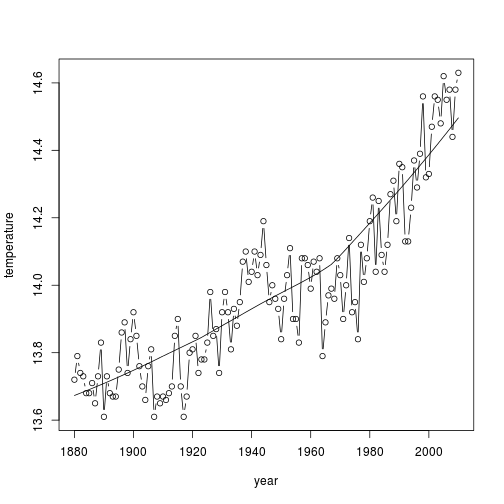
\includegraphics[width=\maxwidth]{figure/unnamed-chunk-2} 

\end{knitrout}


normal quantile plot

\begin{knitrout}
\definecolor{shadecolor}{rgb}{0.969, 0.969, 0.969}\color{fgcolor}\begin{kframe}
\begin{alltt}
\hlkwd{qqnorm}\hlstd{(zz)}
\hlkwd{qqline}\hlstd{(zz)}
\end{alltt}
\end{kframe}
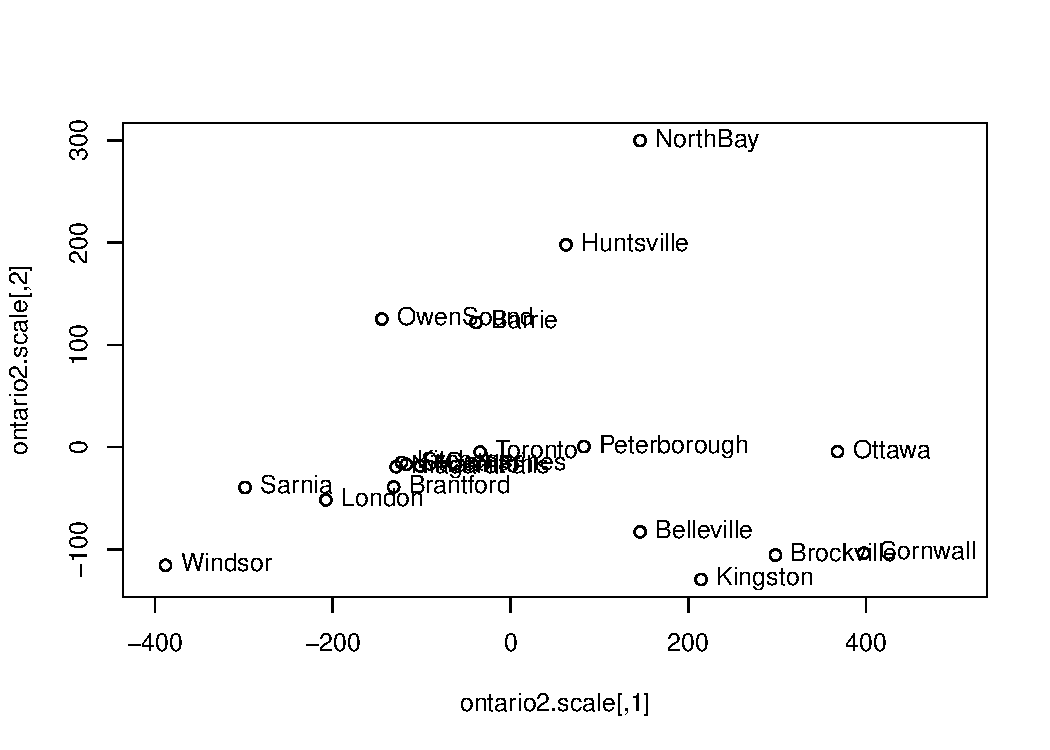
\includegraphics[width=\maxwidth]{figure/unnamed-chunk-3} 

\end{knitrout}


\section{More experimentation}

Some more data:

\begin{knitrout}
\definecolor{shadecolor}{rgb}{0.969, 0.969, 0.969}\color{fgcolor}\begin{kframe}
\begin{alltt}
\hlstd{x} \hlkwb{=} \hlnum{1}\hlopt{:}\hlnum{7}
\hlstd{y} \hlkwb{=} \hlkwd{c}\hlstd{(}\hlnum{10}\hlstd{,} \hlnum{11}\hlstd{,} \hlnum{10}\hlstd{,} \hlnum{13}\hlstd{,} \hlnum{14}\hlstd{,} \hlnum{16}\hlstd{,} \hlnum{19}\hlstd{)}
\end{alltt}
\end{kframe}
\end{knitrout}


Scatterplot, with lowess

\begin{knitrout}
\definecolor{shadecolor}{rgb}{0.969, 0.969, 0.969}\color{fgcolor}\begin{kframe}
\begin{alltt}
\hlkwd{plot}\hlstd{(y} \hlopt{~} \hlstd{x)}
\hlkwd{lines}\hlstd{(}\hlkwd{lowess}\hlstd{(y} \hlopt{~} \hlstd{x))}
\end{alltt}
\end{kframe}
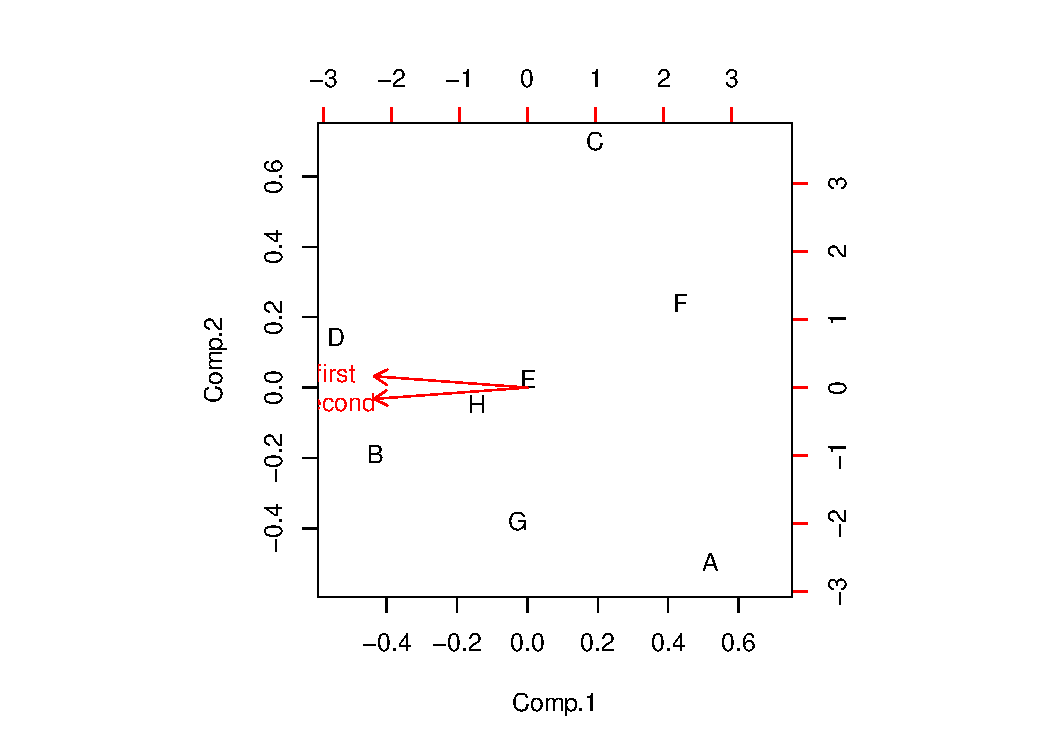
\includegraphics[width=\maxwidth]{figure/unnamed-chunk-5} 

\end{knitrout}


Regression:

\begin{knitrout}
\definecolor{shadecolor}{rgb}{0.969, 0.969, 0.969}\color{fgcolor}\begin{kframe}
\begin{alltt}
\hlstd{y.1} \hlkwb{=} \hlkwd{lm}\hlstd{(y} \hlopt{~} \hlstd{x)}
\hlkwd{summary}\hlstd{(y.1)}
\end{alltt}
\begin{verbatim}
## 
## Call:
## lm(formula = y ~ x)
## 
## Residuals:
##      1      2      3      4      5      6      7 
##  1.107  0.643 -1.821 -0.286 -0.750 -0.214  1.321 
## 
## Coefficients:
##             Estimate Std. Error t value Pr(>|t|)    
## (Intercept)     7.43       1.03    7.23  0.00079 ***
## x               1.46       0.23    6.37  0.00141 ** 
## ---
## Signif. codes:  0 '***' 0.001 '**' 0.01 '*' 0.05 '.' 0.1 ' ' 1
## 
## Residual standard error: 1.22 on 5 degrees of freedom
## Multiple R-squared:  0.89,	Adjusted R-squared:  0.868 
## F-statistic: 40.6 on 1 and 5 DF,  p-value: 0.00141
\end{verbatim}
\begin{alltt}
\hlkwd{par}\hlstd{(}\hlkwc{mfrow} \hlstd{=} \hlkwd{c}\hlstd{(}\hlnum{2}\hlstd{,} \hlnum{2}\hlstd{))}
\hlkwd{plot}\hlstd{(y.1)}
\end{alltt}
\end{kframe}
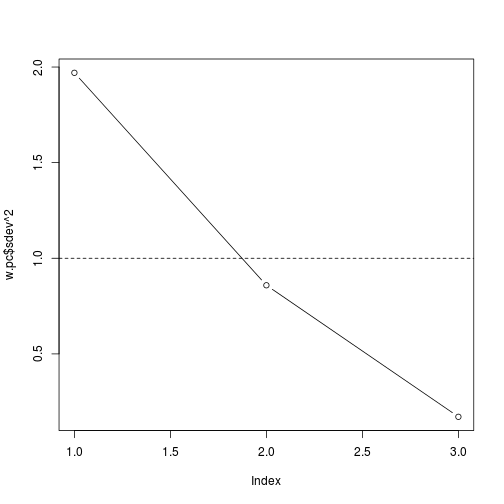
\includegraphics[width=\maxwidth]{figure/unnamed-chunk-6} 

\end{knitrout}


There's a hint of curvature there. Does adding $x^2$ help?

\begin{knitrout}
\definecolor{shadecolor}{rgb}{0.969, 0.969, 0.969}\color{fgcolor}\begin{kframe}
\begin{alltt}
\hlstd{y.2} \hlkwb{=} \hlkwd{lm}\hlstd{(y} \hlopt{~} \hlkwd{poly}\hlstd{(x,} \hlnum{2}\hlstd{))}
\hlkwd{summary}\hlstd{(y.2)}
\end{alltt}
\begin{verbatim}
## 
## Call:
## lm(formula = y ~ poly(x, 2))
## 
## Residuals:
##         1         2         3         4         5         6         7 
## -1.43e-01  6.43e-01 -1.07e+00  7.14e-01  8.25e-16 -2.14e-01  7.14e-02 
## 
## Coefficients:
##             Estimate Std. Error t value Pr(>|t|)    
## (Intercept)   13.286      0.277   48.02  1.1e-06 ***
## poly(x, 2)1    7.748      0.732   10.59  0.00045 ***
## poly(x, 2)2    2.291      0.732    3.13  0.03517 *  
## ---
## Signif. codes:  0 '***' 0.001 '**' 0.01 '*' 0.05 '.' 0.1 ' ' 1
## 
## Residual standard error: 0.732 on 4 degrees of freedom
## Multiple R-squared:  0.968,	Adjusted R-squared:  0.952 
## F-statistic: 60.9 on 2 and 4 DF,  p-value: 0.00101
\end{verbatim}
\begin{alltt}
\hlkwd{par}\hlstd{(}\hlkwc{mfrow} \hlstd{=} \hlkwd{c}\hlstd{(}\hlnum{2}\hlstd{,} \hlnum{2}\hlstd{))}
\hlkwd{plot}\hlstd{(y.2)}
\end{alltt}
\end{kframe}
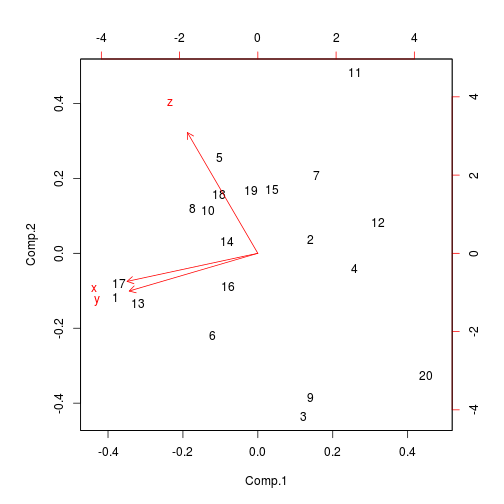
\includegraphics[width=\maxwidth]{figure/unnamed-chunk-7} 

\end{knitrout}


I think it does. Scatterplot of original data with linear and quadratic trends?

\begin{knitrout}
\definecolor{shadecolor}{rgb}{0.969, 0.969, 0.969}\color{fgcolor}\begin{kframe}
\begin{alltt}
\hlkwd{plot}\hlstd{(y} \hlopt{~} \hlstd{x)}
\hlkwd{lines}\hlstd{(x,} \hlkwd{fitted}\hlstd{(y.1),} \hlkwc{col} \hlstd{=} \hlstr{"red"}\hlstd{)}
\hlkwd{lines}\hlstd{(}\hlkwd{spline}\hlstd{(x,} \hlkwd{fitted}\hlstd{(y.2)),} \hlkwc{col} \hlstd{=} \hlstr{"blue"}\hlstd{)}
\end{alltt}
\end{kframe}
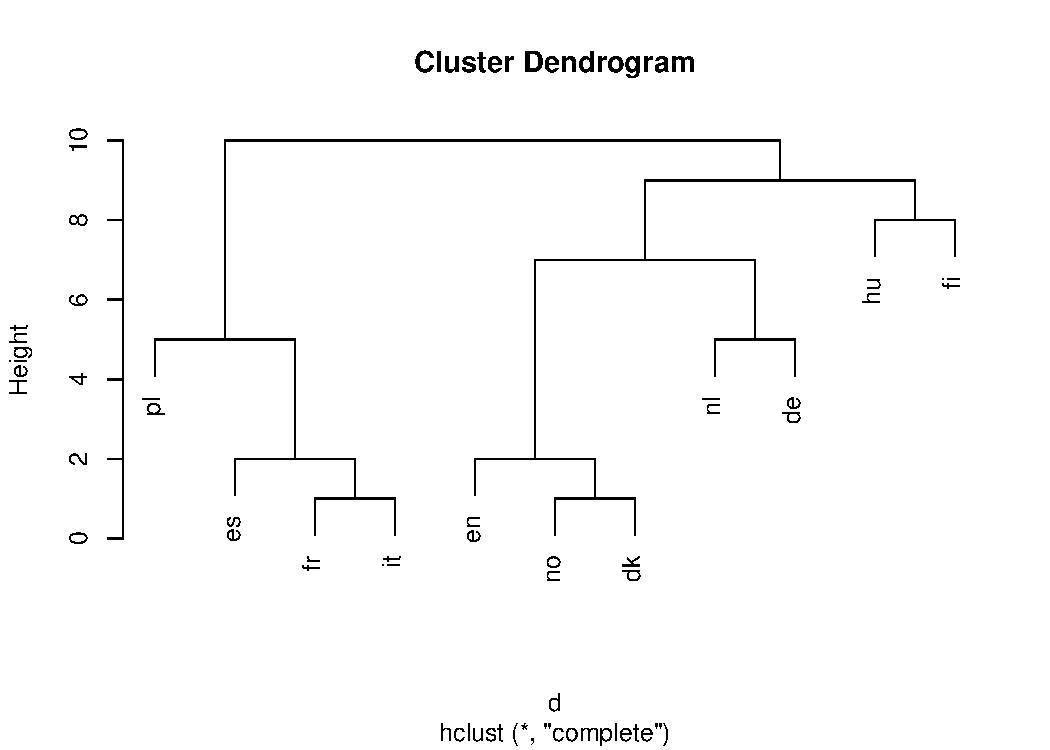
\includegraphics[width=\maxwidth]{figure/unnamed-chunk-8} 

\end{knitrout}


It looks as if the blue curve describes the data better than the red line.
\end{document}
